\documentclass[]{book}
\usepackage{lmodern}
\usepackage{amssymb,amsmath}
\usepackage{ifxetex,ifluatex}
\usepackage{fixltx2e} % provides \textsubscript
\ifnum 0\ifxetex 1\fi\ifluatex 1\fi=0 % if pdftex
  \usepackage[T1]{fontenc}
  \usepackage[utf8]{inputenc}
\else % if luatex or xelatex
  \ifxetex
    \usepackage{mathspec}
  \else
    \usepackage{fontspec}
  \fi
  \defaultfontfeatures{Ligatures=TeX,Scale=MatchLowercase}
\fi
% use upquote if available, for straight quotes in verbatim environments
\IfFileExists{upquote.sty}{\usepackage{upquote}}{}
% use microtype if available
\IfFileExists{microtype.sty}{%
\usepackage{microtype}
\UseMicrotypeSet[protrusion]{basicmath} % disable protrusion for tt fonts
}{}
\usepackage[margin=1in]{geometry}
\usepackage{hyperref}
\hypersetup{unicode=true,
            pdftitle={Class Notes: Intro to Data Science (301033)},
            pdfauthor={Ryan G},
            pdfborder={0 0 0},
            breaklinks=true}
\urlstyle{same}  % don't use monospace font for urls
\usepackage{natbib}
\bibliographystyle{apalike}
\usepackage{color}
\usepackage{fancyvrb}
\newcommand{\VerbBar}{|}
\newcommand{\VERB}{\Verb[commandchars=\\\{\}]}
\DefineVerbatimEnvironment{Highlighting}{Verbatim}{commandchars=\\\{\}}
% Add ',fontsize=\small' for more characters per line
\usepackage{framed}
\definecolor{shadecolor}{RGB}{248,248,248}
\newenvironment{Shaded}{\begin{snugshade}}{\end{snugshade}}
\newcommand{\KeywordTok}[1]{\textcolor[rgb]{0.13,0.29,0.53}{\textbf{#1}}}
\newcommand{\DataTypeTok}[1]{\textcolor[rgb]{0.13,0.29,0.53}{#1}}
\newcommand{\DecValTok}[1]{\textcolor[rgb]{0.00,0.00,0.81}{#1}}
\newcommand{\BaseNTok}[1]{\textcolor[rgb]{0.00,0.00,0.81}{#1}}
\newcommand{\FloatTok}[1]{\textcolor[rgb]{0.00,0.00,0.81}{#1}}
\newcommand{\ConstantTok}[1]{\textcolor[rgb]{0.00,0.00,0.00}{#1}}
\newcommand{\CharTok}[1]{\textcolor[rgb]{0.31,0.60,0.02}{#1}}
\newcommand{\SpecialCharTok}[1]{\textcolor[rgb]{0.00,0.00,0.00}{#1}}
\newcommand{\StringTok}[1]{\textcolor[rgb]{0.31,0.60,0.02}{#1}}
\newcommand{\VerbatimStringTok}[1]{\textcolor[rgb]{0.31,0.60,0.02}{#1}}
\newcommand{\SpecialStringTok}[1]{\textcolor[rgb]{0.31,0.60,0.02}{#1}}
\newcommand{\ImportTok}[1]{#1}
\newcommand{\CommentTok}[1]{\textcolor[rgb]{0.56,0.35,0.01}{\textit{#1}}}
\newcommand{\DocumentationTok}[1]{\textcolor[rgb]{0.56,0.35,0.01}{\textbf{\textit{#1}}}}
\newcommand{\AnnotationTok}[1]{\textcolor[rgb]{0.56,0.35,0.01}{\textbf{\textit{#1}}}}
\newcommand{\CommentVarTok}[1]{\textcolor[rgb]{0.56,0.35,0.01}{\textbf{\textit{#1}}}}
\newcommand{\OtherTok}[1]{\textcolor[rgb]{0.56,0.35,0.01}{#1}}
\newcommand{\FunctionTok}[1]{\textcolor[rgb]{0.00,0.00,0.00}{#1}}
\newcommand{\VariableTok}[1]{\textcolor[rgb]{0.00,0.00,0.00}{#1}}
\newcommand{\ControlFlowTok}[1]{\textcolor[rgb]{0.13,0.29,0.53}{\textbf{#1}}}
\newcommand{\OperatorTok}[1]{\textcolor[rgb]{0.81,0.36,0.00}{\textbf{#1}}}
\newcommand{\BuiltInTok}[1]{#1}
\newcommand{\ExtensionTok}[1]{#1}
\newcommand{\PreprocessorTok}[1]{\textcolor[rgb]{0.56,0.35,0.01}{\textit{#1}}}
\newcommand{\AttributeTok}[1]{\textcolor[rgb]{0.77,0.63,0.00}{#1}}
\newcommand{\RegionMarkerTok}[1]{#1}
\newcommand{\InformationTok}[1]{\textcolor[rgb]{0.56,0.35,0.01}{\textbf{\textit{#1}}}}
\newcommand{\WarningTok}[1]{\textcolor[rgb]{0.56,0.35,0.01}{\textbf{\textit{#1}}}}
\newcommand{\AlertTok}[1]{\textcolor[rgb]{0.94,0.16,0.16}{#1}}
\newcommand{\ErrorTok}[1]{\textcolor[rgb]{0.64,0.00,0.00}{\textbf{#1}}}
\newcommand{\NormalTok}[1]{#1}
\usepackage{longtable,booktabs}
\usepackage{graphicx,grffile}
\makeatletter
\def\maxwidth{\ifdim\Gin@nat@width>\linewidth\linewidth\else\Gin@nat@width\fi}
\def\maxheight{\ifdim\Gin@nat@height>\textheight\textheight\else\Gin@nat@height\fi}
\makeatother
% Scale images if necessary, so that they will not overflow the page
% margins by default, and it is still possible to overwrite the defaults
% using explicit options in \includegraphics[width, height, ...]{}
\setkeys{Gin}{width=\maxwidth,height=\maxheight,keepaspectratio}
\IfFileExists{parskip.sty}{%
\usepackage{parskip}
}{% else
\setlength{\parindent}{0pt}
\setlength{\parskip}{6pt plus 2pt minus 1pt}
}
\setlength{\emergencystretch}{3em}  % prevent overfull lines
\providecommand{\tightlist}{%
  \setlength{\itemsep}{0pt}\setlength{\parskip}{0pt}}
\setcounter{secnumdepth}{5}
% Redefines (sub)paragraphs to behave more like sections
\ifx\paragraph\undefined\else
\let\oldparagraph\paragraph
\renewcommand{\paragraph}[1]{\oldparagraph{#1}\mbox{}}
\fi
\ifx\subparagraph\undefined\else
\let\oldsubparagraph\subparagraph
\renewcommand{\subparagraph}[1]{\oldsubparagraph{#1}\mbox{}}
\fi

%%% Use protect on footnotes to avoid problems with footnotes in titles
\let\rmarkdownfootnote\footnote%
\def\footnote{\protect\rmarkdownfootnote}

%%% Change title format to be more compact
\usepackage{titling}

% Create subtitle command for use in maketitle
\newcommand{\subtitle}[1]{
  \posttitle{
    \begin{center}\large#1\end{center}
    }
}

\setlength{\droptitle}{-2em}

  \title{Class Notes: Intro to Data Science (301033)}
    \pretitle{\vspace{\droptitle}\centering\huge}
  \posttitle{\par}
    \author{Ryan G}
    \preauthor{\centering\large\emph}
  \postauthor{\par}
      \predate{\centering\large\emph}
  \postdate{\par}
    \date{2019-03-13}

\usepackage{booktabs}
\usepackage{amsthm}
\makeatletter
\def\thm@space@setup{%
  \thm@preskip=8pt plus 2pt minus 4pt
  \thm@postskip=\thm@preskip
}
\makeatother

\begin{document}
\maketitle

{
\setcounter{tocdepth}{1}
\tableofcontents
}
\chapter{Prerequisites}\label{prerequisites}

These are topic Notes and Practicals for IntrotoDataSci, the material
is:

\begin{longtable}[]{@{}ll@{}}
\toprule
Week no. & Topic\tabularnewline
\midrule
\endhead
1 & Introduction to Data Science\tabularnewline
2 & Supervised Learning: Linear Models 1\tabularnewline
3 & Supervised Learning: Linear Models 2\tabularnewline
4 & Supervised Learning: Classification (Logistic
Regression)\tabularnewline
5 & Resampling Methods (e.g.~Cross-Validation, Training Split
etc.)\tabularnewline
6 & Supervised Learning: Tree Based Methods\tabularnewline
7 & Supervised learning: Classification (Support Vector
Machines)\tabularnewline
8 & unsupervised learning: Principal Component Analysis\tabularnewline
9 & STUVAC\tabularnewline
10 & Unsupervised Learning: Clustering\tabularnewline
11 & Guest Lecture\tabularnewline
12 & Guest Lecture\tabularnewline
13 & Revision\tabularnewline
14 & Final Exam\tabularnewline
\bottomrule
\end{longtable}

In this unit we will cover:

\begin{itemize}
\tightlist
\item
  Supervised learning:

  \begin{itemize}
  \tightlist
  \item
    Linear Models
  \item
    Classification (KNN and Discrimination)
  \item
    Classification and Regression Trees
  \end{itemize}
\item
  Unsupervised Learning:

  \begin{itemize}
  \tightlist
  \item
    DimensionReduction: Principal Component Analysis
  \item
    Clustering: K Means and Hierarchical
  \end{itemize}
\item
  Unstrucutred Data:

  \begin{itemize}
  \tightlist
  \item
    Text Mining
  \end{itemize}
\item
  Resampling
\item
  Visualisation
\end{itemize}

\chapter{(Wk 1) Introduction to Data
Science}\label{wk-1-introduction-to-data-science}

Material of 5 March 2019, week 1 test \#\# Types of Data Data is
classified as either structured or unstructured:

\begin{itemize}
\tightlist
\item
  \textbf{\emph{Structured Data}}

  \begin{itemize}
  \tightlist
  \item
    \textbf{Quantitative}/Numeric Data

    \begin{itemize}
    \tightlist
    \item
      Height, Weight, Salary etc.
    \end{itemize}
  \item
    Qualitative Data (also known as Categorical Data, Factors, or
    Discrete Variables)

    \begin{itemize}
    \tightlist
    \item
      be careful, factors usually refer to the variables in a predictive
      model
    \item
      When dealing with factors in
      
\includegraphics{./images/Ricon20px.png} it is necessary to use a
      data type called factors discussed below

      \begin{itemize}
      \tightlist
      \item
        Examples of categorical data include alive/dead, male/femaile,
        ethnicity, product code, hair colour etc.
      \end{itemize}
    \end{itemize}
  \end{itemize}
\end{itemize}

\subsection[Categorical variables in ]{\texorpdfstring{Categorical
variables in
\protect
\includegraphics{images/Ricon40px.png}}{Categorical variables in }}\label{categorical-variables-in}

In order to deal with discrete variables

\includegraphics{images/Ricon20px.png} uses a data type called factors,
to create factors the \texttt{factor()} command is used, within this
command a vector containing factor levels must be enclosed, e.g.

\begin{Shaded}
\begin{Highlighting}[]
\KeywordTok{factor}\NormalTok{(}\KeywordTok{c}\NormalTok{(}\StringTok{"Male"}\NormalTok{, }\StringTok{"Female"}\NormalTok{))}
\end{Highlighting}
\end{Shaded}

\begin{verbatim}
## [1] Male   Female
## Levels: Female Male
\end{verbatim}

\subsubsection{Categorical Variables and
Regression}\label{categorical-variables-and-regression}

When performing a multiple linear regression with categorical data, the
cqategorical data will be treated as a boolean \texttt{1/0} variable,
basically choosing between different categorical variables is choosing a
different intercept for the regression (i.e.~adding a constant value)

\begin{quote}
under the hood 1 corresponds to True and 0 corresponds to false
\end{quote}

\paragraph{Not as accurate}\label{not-as-accurate}

This is not as accurate as using a linear regression seperately on the
data within that category, so, unless there is a good reason i.e.~the
different categories would have a trend with the same rate but a
different intercept, e.g.~the ambient temperature of a location would
have different mean values for each month:

\[
\text{Response} = -74 = 3.109 \cdot X_{\text{wind}} - 1.875\cdot X_{\text{temp}} + 14.76 \cdot \left( \text{Jan} \right) + 8.75 \cdot \left( \text{Feb} \right) +4.197 \cdot \left( \text{Mar}) \right) 
\]

in this case \(\text{Jan}\), \(\text{Feb}\) etc. would be a
\texttt{True}/\texttt{False} (\(\equiv\) \texttt{1}/\texttt{0}) value
indicating whether or not to include that constant in the equation
(because it is or isn't that date) so if in this example Sydney is an
everage of 23 degrees, maybe January is on average 14 degrees hotter and
the coefficient for July might be -14 because in July it is 14 degrees
cooler.

\section{Supervised vs Unsupervised
Problems}\label{supervised-vs-unsupervised-problems}

Machine Learning problems are often split into two categories,
supervised and unsupervised.

\textbf{Supervised Learning} involves data where each observational unit
has one special variable, (e.g.~survive/perish, amount spent).

\textbf{Unsupervised Learning} Is about pattern discovery, there is no
clear special variable (e.g.~trying to detect unusual spending or
grouping spenders into seperate groups).

\subsection{Supervised Learning}\label{supervised-learning}

Supervised Learning has a response variable (also known as outcome or in
calculus as an independent variable, \(Y\)) and the idea is to
predicting the relationship between the output and several inputs:

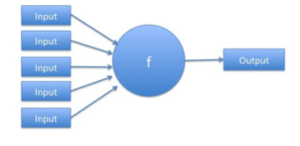
\includegraphics{images/supfunc300px.jpg}
knitr::include\_graphics(rep(``images/knit-logo.png'', 3))

In a classification problem \(Y\) takes the value of a discrete variable
(e.g.~survived/perished), In a regression problem \(Y\) takes a
\(\mathbb{R}\) quantitative value (e.g. \(\$72.45\) or
\(55 \text{ kg}\))

In Mathematical terms, if \(y\) was the output and
\(x_1, x_2, x_3 \dots\) the input, the model would be the expected value
of \(y\) given the inputs, denoted \(E(y)\), defined by some function
\(f\):

\[
E(y) = f(x_1, x_2, x_3, \dots)
\]

The observed output is expected to vary in value owing to errors in
measurement (so for example even though we have very strong mathematical
evidence for a relationship, e.g. \(S = \frac{1}{2}at^2)\) we would
expect the observed values to contain error.

\begin{Shaded}
\begin{Highlighting}[]
\NormalTok{n <-}\StringTok{ }\DecValTok{100}
\NormalTok{x <-}\StringTok{ }\DecValTok{1}\OperatorTok{:}\NormalTok{n}
\NormalTok{y <-}\StringTok{ }\FloatTok{0.5}\OperatorTok{*}\FloatTok{9.81}\OperatorTok{*}\NormalTok{x}\OperatorTok{^}\DecValTok{2} \OperatorTok{+}\StringTok{ }\KeywordTok{rnorm}\NormalTok{(n, }\DataTypeTok{mean =} \DecValTok{0}\NormalTok{, }\DataTypeTok{sd =} \DecValTok{2000}\NormalTok{)}

\NormalTok{##layout(matrix(1:2, ncol =2))}

\CommentTok{#Using baseplot}

  \CommentTok{#model <- lm(y ~ poly(x, degree = 2))}
  \CommentTok{#plot(y~x)}
  \CommentTok{#Expy <- predict(object = model)}
  \CommentTok{#lines(Expy)}

\CommentTok{#Using GGplot2}
\NormalTok{egdata <-}\StringTok{ }\KeywordTok{data.frame}\NormalTok{(}\DataTypeTok{height =}\NormalTok{ y, }\DataTypeTok{time =}\NormalTok{ x) }\CommentTok{#create dataframe}
\KeywordTok{ggplot}\NormalTok{(}\DataTypeTok{data =}\NormalTok{ egdata, }\KeywordTok{aes}\NormalTok{(}\DataTypeTok{x =}\NormalTok{ time, }\DataTypeTok{y =}\NormalTok{ height)) }\OperatorTok{+}\StringTok{ }\CommentTok{# call ggplot2}
\StringTok{  }\KeywordTok{geom_point}\NormalTok{(}\DataTypeTok{col =} \StringTok{"#7f7caf"}\NormalTok{, }\DataTypeTok{size =} \DecValTok{3}\NormalTok{, }\DataTypeTok{alpha =} \FloatTok{0.5}\NormalTok{) }\OperatorTok{+}\StringTok{ }\CommentTok{#plot the points for the data}
\StringTok{  }\KeywordTok{stat_smooth}\NormalTok{(}\DataTypeTok{col =} \StringTok{"#7d2e68"}\NormalTok{, }\DataTypeTok{method =} \StringTok{'lm'}\NormalTok{, }\DataTypeTok{formula =}\NormalTok{ y }\OperatorTok{~}\StringTok{ }\KeywordTok{poly}\NormalTok{(x, }\DecValTok{2}\NormalTok{, }\DataTypeTok{raw =} \OtherTok{TRUE}\NormalTok{), }\DataTypeTok{se =} \OtherTok{FALSE}\NormalTok{) }\OperatorTok{+}\StringTok{ }\CommentTok{# draw the polynomial model}
\StringTok{  }\KeywordTok{theme_classic}\NormalTok{() }\CommentTok{# change the theme}
\end{Highlighting}
\end{Shaded}

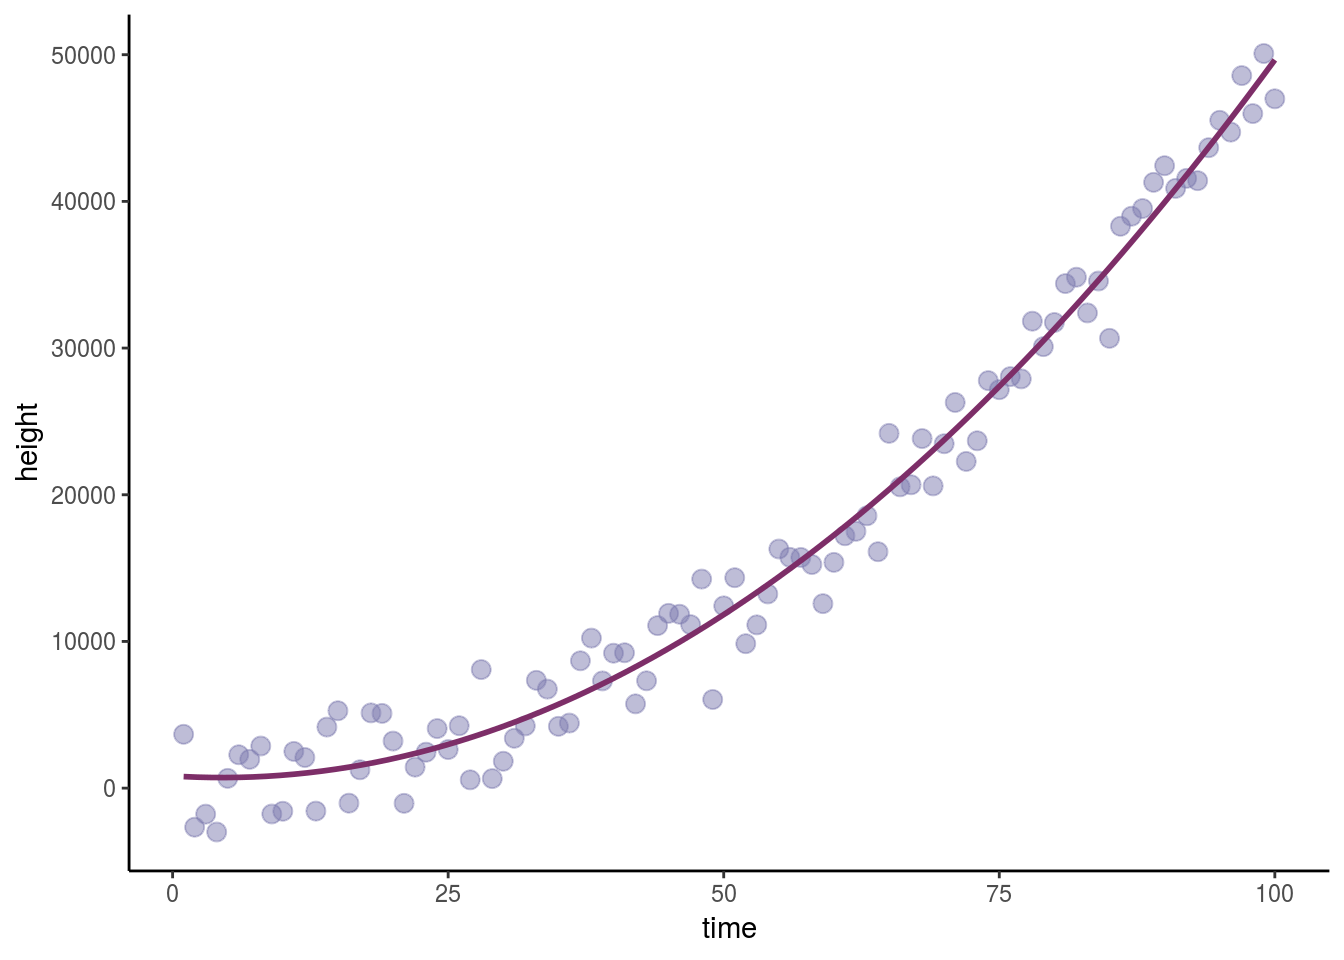
\includegraphics[width=0.4\linewidth]{bookdown-demo_files/figure-latex/unnamed-chunk-3-1}

\begin{Shaded}
\begin{Highlighting}[]
  \CommentTok{# use https://coolors.co/app for colour themes}
\end{Highlighting}
\end{Shaded}

\subsubsection{Types of Errors (Stochastic
Trends)}\label{types-of-errors-stochastic-trends}

\begin{itemize}
\tightlist
\item
  Random Error

  \begin{itemize}
  \tightlist
  \item
    unforseeable fluctuations in Data
  \end{itemize}
\item
  Systemic Error

  \begin{itemize}
  \tightlist
  \item
    Shortcomings of the capacity to measure accurately

    \begin{itemize}
    \tightlist
    \item
      e.g.~Measuring using a ruler that is \(\pm1 \text{ mm}\)
    \end{itemize}
  \end{itemize}
\end{itemize}

\subsubsection{Choosing the right Model}\label{choosing-the-right-model}

It's also necessary to choose the right type of model, for example below
the function chosen on the left is a simple linear regression, but maybe
it's appropriate to assume that there is a seasonal or cyclical trend (a
cyclical trend being less predictable like a recession and a seasonal
being more predictable like seasons).

\begin{figure}
\centering
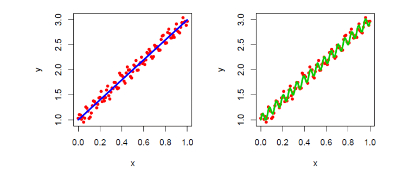
\includegraphics{images/Cycvsseas400px.jpg}
\caption{Comparison of more complex and simpler models}
\end{figure}

\subsubsection{Bias and Variance}\label{bias-and-variance}

The more complex a function, the more variance in fitting that function
(because there is more uncertainty around the fitted parameters).
However fitting a simpler function can introduce more bias because there
may be a more fundamental difference between the predicted and actual
values.

\subsubsection{Model Evaluation}\label{model-evaluation}

Prediction accuracy is estimated from the same sample that was used to
fit the function, two strategies are used to offset the bias that this
would introduce:

\begin{itemize}
\tightlist
\item
  Splitting the Data

  \begin{itemize}
  \tightlist
  \item
    Use \textbf{training data} to create the model
  \item
    \textbf{validation data} to validate the model accuracy
  \item
    \textbf{testing data} to measure the accuracy of the model
    predictions
  \end{itemize}
\item
  Cross Validation

  \begin{itemize}
  \tightlist
  \item
    Cross Validation only tests the modelling process while splitting
    the data evaluates the final model
  \end{itemize}
\end{itemize}

\subsubsection{Classification and
Regression}\label{classification-and-regression}

\paragraph{Regression}\label{regression}

When the output is a numeric variable, supervised learning can be
referred to as regression, some examples of regression are:

\begin{itemize}
\tightlist
\item
  Linear Regression (Simple or Multiple)
\item
  Generalised Linear Models (\texttt{glm})
\item
  Neural Networks

  \begin{itemize}
  \tightlist
  \item
    Neural Networks is an example of a non-paramentric method, the above
    two rely on statistical assumptions
  \end{itemize}
\end{itemize}

\paragraph{Classification}\label{classification}

When the output is a categorical variable supervised learning is known
as classification

\begin{itemize}
\tightlist
\item
  K-Nearest Neighbours
\item
  Generalised Linear Models (Logistic Regression)
\end{itemize}

\subsection{Unsupervised Problems}\label{unsupervised-problems}

When there is no output variable the problem is usually one of
\textbf{unsupervised Learning} a common example is clustering data, for
example:

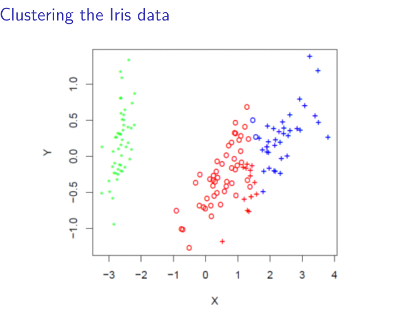
\includegraphics{images/clust400px.jpg} In this example the goal would
be to classify the data according to the colours.

In this unit we will cover:

\begin{itemize}
\tightlist
\item
  Supervised learning:

  \begin{itemize}
  \tightlist
  \item
    Linear Models
  \item
    Classification (KNN and Discrimination)
  \item
    Classification and Regression Trees
  \end{itemize}
\item
  Unsupervised Learning:

  \begin{itemize}
  \tightlist
  \item
    DimensionReduction: Principal Component Analysis
  \item
    Clustering: K Means and Hierarchical
  \end{itemize}
\item
  Unstrucutred Data:

  \begin{itemize}
  \tightlist
  \item
    Text Mining
  \end{itemize}
\item
  Resampling
\item
  Visualisation
\end{itemize}

\chapter{(Wk 2) Introduction to Data
Science}\label{wk-2-introduction-to-data-science}

Material of Tue 12 2019, week 2 test

\section{Heading 1}\label{heading-1}

\subsection{Sub Heading 1}\label{sub-heading-1}

\section{Heading 2}\label{heading-2}

\subsection{Sub Heading 1}\label{sub-heading-1-1}

\section{Heading 3}\label{heading-3}

\subsection{Sub Heading 1}\label{sub-heading-1-2}

\chapter{(Wk 3) Introduction to Data
Science}\label{wk-3-introduction-to-data-science}

Material of Tue 19 March2019, week 3 testlkj

\section{Heading 1}\label{heading-1-1}

\subsection{Sub Heading 1}\label{sub-heading-1-3}

\section{Heading 2}\label{heading-2-1}

\subsection{Sub Heading 1}\label{sub-heading-1-4}

\section{Heading 3}\label{heading-3-1}

\subsection{Sub Heading 1}\label{sub-heading-1-5}

\chapter{(Wk 4) Introduction to Data
Science}\label{wk-4-introduction-to-data-science}

Material of Tue 26 March 2019, week 4

\section{Heading 1}\label{heading-1-2}

\subsection{Sub Heading 1}\label{sub-heading-1-6}

\section{Heading 2}\label{heading-2-2}

\subsection{Sub Heading 1}\label{sub-heading-1-7}

\section{Heading 3}\label{heading-3-2}

\subsection{Sub Heading 1}\label{sub-heading-1-8}

\chapter{(Wk 5) Introduction to Data
Science}\label{wk-5-introduction-to-data-science}

Material of Tue 2 April 2019, week 5

\section{Heading 1}\label{heading-1-3}

\subsection{Sub Heading 1}\label{sub-heading-1-9}

\section{Heading 2}\label{heading-2-3}

\subsection{Sub Heading 1}\label{sub-heading-1-10}

\section{Heading 3}\label{heading-3-3}

\subsection{Sub Heading 1}\label{sub-heading-1-11}

\chapter{(Wk n) Introduction to Data
Science}\label{wk-n-introduction-to-data-science}

Material of Tue 9 April 2019, week 6

\section{Heading 1}\label{heading-1-4}

\subsection{Sub Heading 1}\label{sub-heading-1-12}

\section{Heading 2}\label{heading-2-4}

\subsection{Sub Heading 1}\label{sub-heading-1-13}

\section{Heading 3}\label{heading-3-4}

\subsection{Sub Heading 1}\label{sub-heading-1-14}

\chapter{(Wk n) Introduction to Data
Science}\label{wk-n-introduction-to-data-science-1}

Material of Tue 16 April 2019, week 7

\section{Heading 1}\label{heading-1-5}

\subsection{Sub Heading 1}\label{sub-heading-1-15}

\section{Heading 2}\label{heading-2-5}

\subsection{Sub Heading 1}\label{sub-heading-1-16}

\section{Heading 3}\label{heading-3-5}

\subsection{Sub Heading 1}\label{sub-heading-1-17}

\chapter{(Wk 8) Introduction to Data
Science}\label{wk-8-introduction-to-data-science}

Material of Tue 23 April 2019, week 8

\section{Heading 1}\label{heading-1-6}

\subsection{Sub Heading 1}\label{sub-heading-1-18}

\section{Heading 2}\label{heading-2-6}

\subsection{Sub Heading 1}\label{sub-heading-1-19}

\section{Heading 3}\label{heading-3-6}

\subsection{Sub Heading 1}\label{sub-heading-1-20}

\chapter{(Wk 10) Introduction to Data
Science}\label{wk-10-introduction-to-data-science}

Material of Tue 6 May 2019, week 10

\section{Heading 1}\label{heading-1-7}

\subsection{Sub Heading 1}\label{sub-heading-1-21}

\section{Heading 2}\label{heading-2-7}

\subsection{Sub Heading 1}\label{sub-heading-1-22}

\section{Heading 3}\label{heading-3-7}

\subsection{Sub Heading 1}\label{sub-heading-1-23}

\chapter{(Wk 11) Introduction to Data
Science}\label{wk-11-introduction-to-data-science}

Material of Tue 13 May 2019, week 11

\section{Heading 1}\label{heading-1-8}

\subsection{Sub Heading 1}\label{sub-heading-1-24}

\section{Heading 2}\label{heading-2-8}

\subsection{Sub Heading 1}\label{sub-heading-1-25}

\section{Heading 3}\label{heading-3-8}

\subsection{Sub Heading 1}\label{sub-heading-1-26}

\chapter{(Wk 12) Introduction to Data
Science}\label{wk-12-introduction-to-data-science}

Material of Tue 20 May 2019, week 12

\section{Heading 1}\label{heading-1-9}

\subsection{Sub Heading 1}\label{sub-heading-1-27}

\section{Heading 2}\label{heading-2-9}

\subsection{Sub Heading 1}\label{sub-heading-1-28}

\section{Heading 3}\label{heading-3-9}

\subsection{Sub Heading 1}\label{sub-heading-1-29}

\chapter{(Wk 13) Introduction to Data
Science}\label{wk-13-introduction-to-data-science}

Material of Tue 27 May 2019, week 13

\section{Heading 1}\label{heading-1-10}

\subsection{Sub Heading 1}\label{sub-heading-1-30}

\section{Heading 2}\label{heading-2-10}

\subsection{Sub Heading 1}\label{sub-heading-1-31}

\section{Heading 3}\label{heading-3-10}

\subsection{Sub Heading 1}\label{sub-heading-1-32}

\bibliography{book.bib,packages.bib}


\end{document}
